%================================================================
\section{Results and Discussion}\label{sec:Results}
%================================================================

The procedures for producing the following results are contained in Jupyter Notebooks found here:
\begin{center}
    \url{https://github.com/nicolossus/FYS-STK4155-Project2/tree/master/notebooks}
\end{center}

The associated source code can similarly be found here: 
\begin{center}
    \url{https://github.com/nicolossus/FYS-STK4155-Project2/tree/master/src}
\end{center}

%----------------------------------------------------------------
\subsection{Producing Data for 1D Ising Model}\label{sec:results datagen}
%----------------------------------------------------------------

Discuss counting in the all-to-all Ising model

%----------------------------------------------------------------
\subsection{Learning the Ising Hamiltonian with Linear Regression}\label{sec:results linreg}
%----------------------------------------------------------------

\begin{figure}[H]
\centering
\subfloat[]{{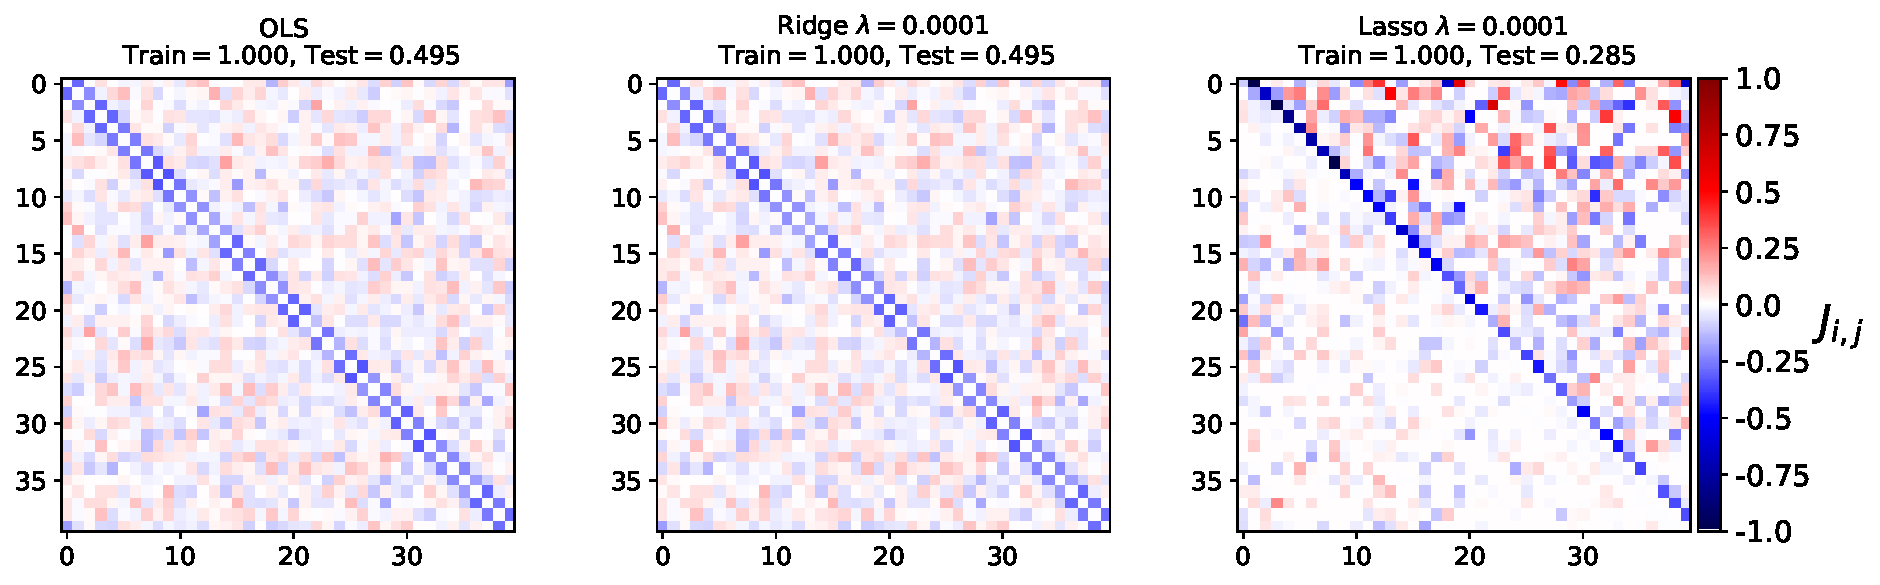
\includegraphics[scale=0.5]{latex/figures/ising_J_lmbda_0_0001.pdf}}}
\qquad
\subfloat[]{{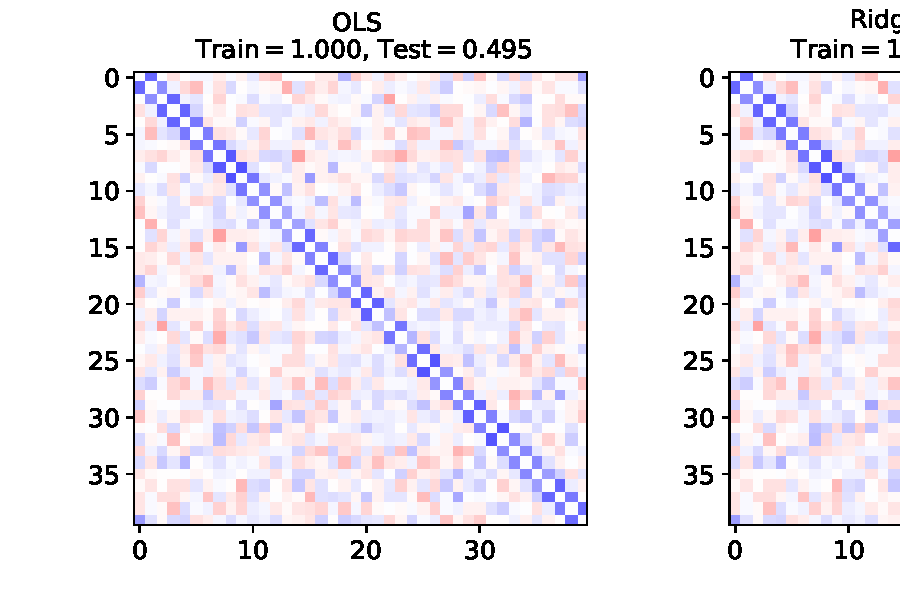
\includegraphics[scale=0.5]{latex/figures/ising_J_lmbda_0_001.pdf}}}
\qquad
\subfloat[]{{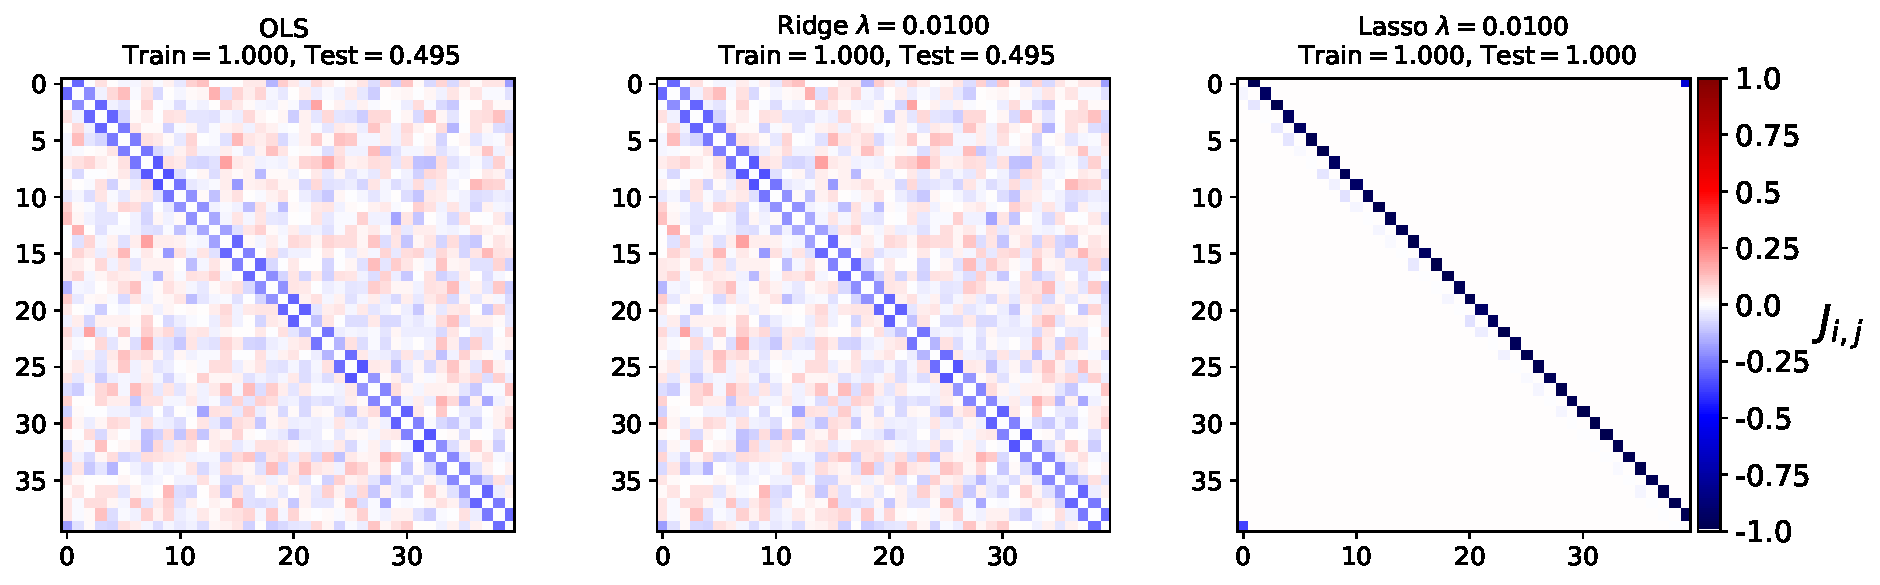
\includegraphics[scale=0.5]{latex/figures/ising_J_lmbda_0_01.pdf}}}
\caption{figure text}
\label{fig:fig1}
\end{figure}


%----------------------------------------------------------------
\subsection{Identifying 2D Ising Model Phases with Logistic Regression}\label{sec:results logreg}
%----------------------------------------------------------------

%----------------------------------------------------------------
\subsection{Identifying 2D Ising Model Phases with Neural Networks}\label{sec:results NN}
%----------------------------------------------------------------